% ====================================================================
%+
% SECTION:
%    supernovacosmology.tex
%
% CHAPTER:
%    cosmology.tex
%
% ELEVATOR PITCH:
%    SNIa cosmology, approach to evaluating dependence of science on cadence
%
% COMMENTS:
%
%
% BUGS:
%
%
% AUTHORS:
%    Phil Marshall (@drphilmarshall)  - put your name and GitHub username here!
%-
% ====================================================================
\clearpage
\newpage

\section{Supernova Cosmology and Physics}
\def\secname{supernovae}\label{sec:\secname}
% \label{sec:cosmology, supernovae, classification, lenstimedelays, deepdrillingfields }

\noindent{\it Jeonghee Rho, Michelle Lochner, Rahul Biswas, Seth Digel} % (Writing team)

% This individual section will need to describe the particular
% discoveries and measurements that are being targeted in this section's
% science case. It will be helpful to think of a ``science case" as a
% ``science project" that the authors {\it actually plan to do}. Then,
% the sections can follow the tried and tested format of an observing
% proposal: a brief description of the investigation, with references,
% followed by a technical feasibility piece. This latter part will need
% to be quantified using the MAF framework, via a set of metrics that
% need to be computed for any given observing strategy to quantify its
% impact on the described science case. Ideally, these metrics would be
% combined in a well-motivated figure of merit. The section can conclude
% with a discussion of any risks that have been identified, and how
% these could be mitigated.

This section is concerned with the detection and characterization of
supernovae (SNe) over time with LSST and their various scientific
applications. A crucial application is the use of supernovae type
Ia (SNIa) and potentially some core-collapse SN (like type IIP) to trace
the recent expansion history of the universe, and confront models of the
physics driving the late time accelerated expansion of the universe.

This objective of SN cosmology follows (at least for SNIa) results from
several highly successful surveys; improvement in knowledge of cosmology
could come from substantially larger numbers of well-characterized SNe.
This goal is not directly tied to the unprecedentedly large survey area of
LSST; the larger number of well-characterized supernovae may be obtained from
a relatively smaller spatio-temporal region with larger numbers of light curves
well characterized. However, in practice, even this goal could
benefit from the spatial scale offered by the WFD component of the LSST
survey. 

On the other hand, the WFD aspect will make the LSST survey potentially the
first to scan the very large area of the entire Southern sky for SNe. SNe
that are detected and well characterized by LSST can trace large scale
large scale structure (albeit more noisily than galaxies due to smaller numbers) and includes estimates of radial distances, and their own redshift estimates which may be used in conjunction with host galaxy redshift information. Due to
these properties they will probe the isotropy of the late time universe. 
Peculiar velocities of SNe will probe the growth of structure.  In addition, this large sample will enable further sharpening
of our understanding of the properties of the SN population of different
types. This last point is extremely important for SN cosmology goals:  The
success of SNIa cosmology has always been based on the empirical model that
intrinsic peak brightnesses are related to the certain observable
characteristics of SNe. 
The WFD SNIa sample will dramatically increase the size of the sample
available to train such an empirical model, as well understand the
probability of deviations and scatter from this model. Aside from issues
like calibration which need to be addressed differently, a larger sample of
such well measured SNe is probably the only way to address `systematics'
due to deviations from the empirical model. The anticipated sample can be
thought of as consisting of two components:  the low-redshift sample which
is more likely to be complete, and the higher-redshift sample that will be
able to constrain evolution. 

% --------------------------------------------------------------------

\subsection{Target measurements and discoveries}
\label{sec:\secname:targets}

% Describe the discoveries and measurements you want to make.

SNe of different types are visible over time scales of about a few 
weeks (e.g., type Ia) to nearly a year (type IIP).  During the full ten-year
 survey, LSST will scan the entire southern sky repeatedly
 with a WFD cadence, and certain specific locations
of the sky called the Deep Drilling Fields (DDF) with special enhanced cadence. 

This spatio-temporal window should contain millions \todo{RB}{remember to
check} of SNe, that will have apparent magnitudes brighter than the single
exposure limiting magnitude of LSST.  However, the actual sequence of
observations by LSST, defined by the series of field pointing as a
function of time in filter bands (along with weather conditions), will
determine the extent to which each SN can be detected and characterized
well.  Characterization of the SNe is at the core of a number of science
programs that use them as bright, abundant objects with empirically
determined intrinsic brightnesses. For LSST, this goal entails (a)
detection of SNe, (b) photometric typing of SNe, (c) estimating photometric
redshifts of SNe (or identifying host galaxies and obtaining their
redshifts from photometry or follow-up spectroscopy), (d) estimation of
intrinsic brightnesses of the SNe, and finally (e) use of these data in
addressing our science goals of cosmological inference, etc. The efficacy
of photometric typing, redshifts and estimation of intrinsic brightnesses
are all dependent on the amount of information available in the observed
light curves of SNe. While these steps are not necessarily independent, it
is useful to think of the requirements on some of these steps separately;
it is not unlikely  that combinations of some of the steps would still be
affected by similar requirements. 

{\emph{Our first objective is to detect such SNe}}, by which we mean
selecting SNe from among the transient sources detected by LSST.
% classify them as SNe (as opposed to an AGN, or an asteroid). 
In brief, this process consists of defining a set of image subtractions
between a high-resolution `template` image of a sky section, and a set of
single exposures at different times (usually of lower resolution) of the
same region, after accounting for the different resolutions of images, and
alignments. These sets of image subtractions associated with a single
object will be used to detect the object as a transient and then classify
the transient as an SN. Clearly, detecting an SN depends on the number of
such images recorded per object, the different filters used for those
images, and the signal-to-noise ratios of the images. %One might expect
The efficiency of this step may be summarized as a threshold on the
joint properties of an astrophysical candidate (apparent brightness, light
curve characteristics, background) as well as observing conditions
(astronomical seeing, etc.).  

{\emph{Our second objective is to photometrically classify different kinds of SNe.}} 
%{\bfseries Photometric SN classification}\\
Previously, only spectroscopically typed SNe have been used for cosmology. Photometric 
typing from light curves alone has only been used to select candidates for spectroscopic 
follow-up (see, e.g., \citet{Sako2008}). However, LSST will simply find far too many 
candidates for even a significant fraction of them to be followed up spectroscopically. In order to avoid 
discarding the majority of the SN dataset, we need to use techniques capable of 
determining cosmological parameters from a potentially contaminated photometric SN dataset.

Several techniques have been proposed recently to solve this problem. One 
approach involves applying stringent cuts to the photometric dataset to obtain a nearly pure sample 
of SNIa \citep{Bernstein2012,Campbell2013} and running the standard SNIa cosmology analysis 
with this sample. Another approach, BEAMS \citep{Kunz2007,Newling2011,Hlozek2012,Knights2013}, 
makes use of an entire dataset, coping with contamination by using a mixture model for the 
likelihood, thus allowing for multiple populations. Whichever the technique ultimately used for 
cosmological analysis, it will rely on accurate initial classifications of SN type and 
unbiased estimates for the probability of each type.

Current state-of-the-art photometric classification techniques rely on
fitting empirically determined templates of SNe to light curves
\citep{Jha2007,Guy2007,Sako2011}. However in recent years, new approaches
have been developed in response to the 2010 `Supernova Photometric
Classification Challenge' \citep{Kessler2010a}. Many of these use novel
light curve parameterization and employ machine learning algorithms to
perform the classification (see \citet{Kessler2010b} and references
therein).

While many of these methods have been tested on standard sets of simulated data and (in some cases) 
on SDSS data, which technique (if any) is superior in all situations is unclear. For 
example, some techniques are more dependent than others on the availability of reliable redshift information, and how 
these techniques will respond to changes in cadence, filter sets, signal-to-noise, 
etc., is unclear.  

With this in mind, we propose the use of a multifaceted classification system which
employs several different methods for extracting features from the light curves (e.g.,
fitting parametric functions or templates) and several different classification
algorithms. This system is highly modular, allowing new approaches for direct comparison
with existing  techniques to be added easily. This also allows direct analysis of
different observing strategies, without requiring an initial choice of classification
technique.


{\emph{Our third objective is to characterize SNe in terms of empirical
    light curve models.}}

The ultimate goal of using SNe (type SNIa or SNIIP) for cosmology requires estimating the
intrinsic brightnesses of the SN. The first (and sometimes only, depending on the light
curve model) step is fitting the calibrated fluxes to a light curve model with a set of
parameters. According to the ansatz used in SN cosmology, the intrinsic brightness of SNe
is largely determined by the parameters of the light curve model; hence the uncertainties
on the inferred parameters largely determine the uncertainties on the inferred peak
intrinsic brightness or distance moduli of the SNe.

% Now, describe their response to the observing strategy. Qualitatively,
% how will the science project be affected by the observing schedule and
% conditions? 

% In broad terms, how would we expect the observing strategy
% to be optimized for this science?





% --------------------------------------------------------------------

\subsection{Metrics}
\label{sec:\secname:metrics}

{\it Quantifying the response via MAF metrics: definition of the metrics,
and any derived overall figure of merit.}
\label{sec:\secname:metrics}
\begin{figure}
 \centering
 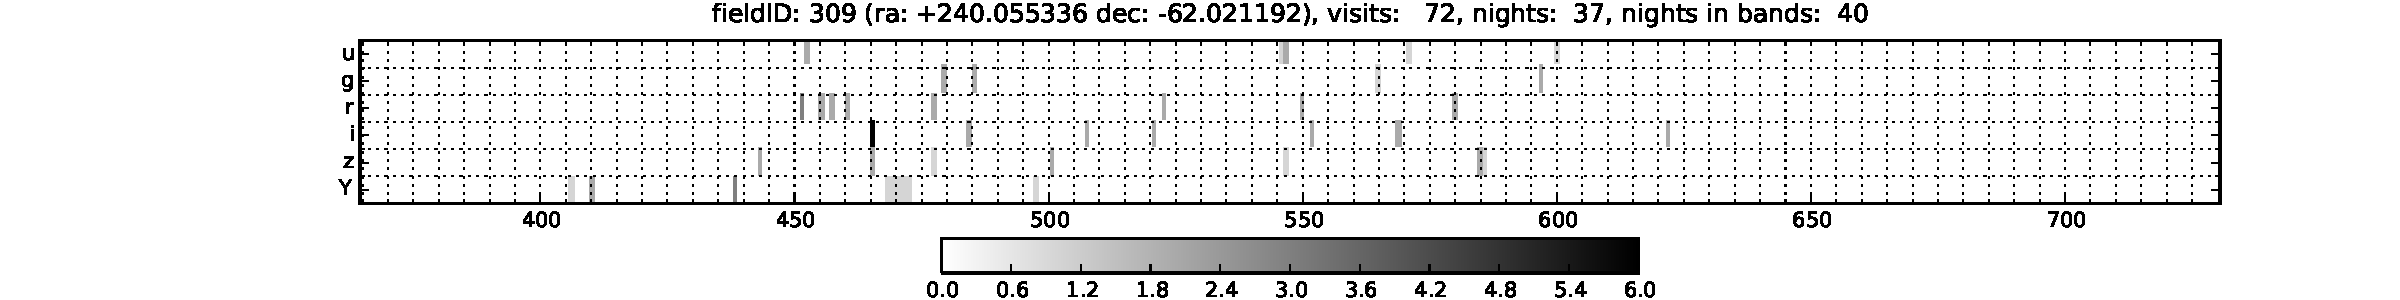
\includegraphics[width=\textwidth]{figs/supernova/fig_309_2ndYear}
 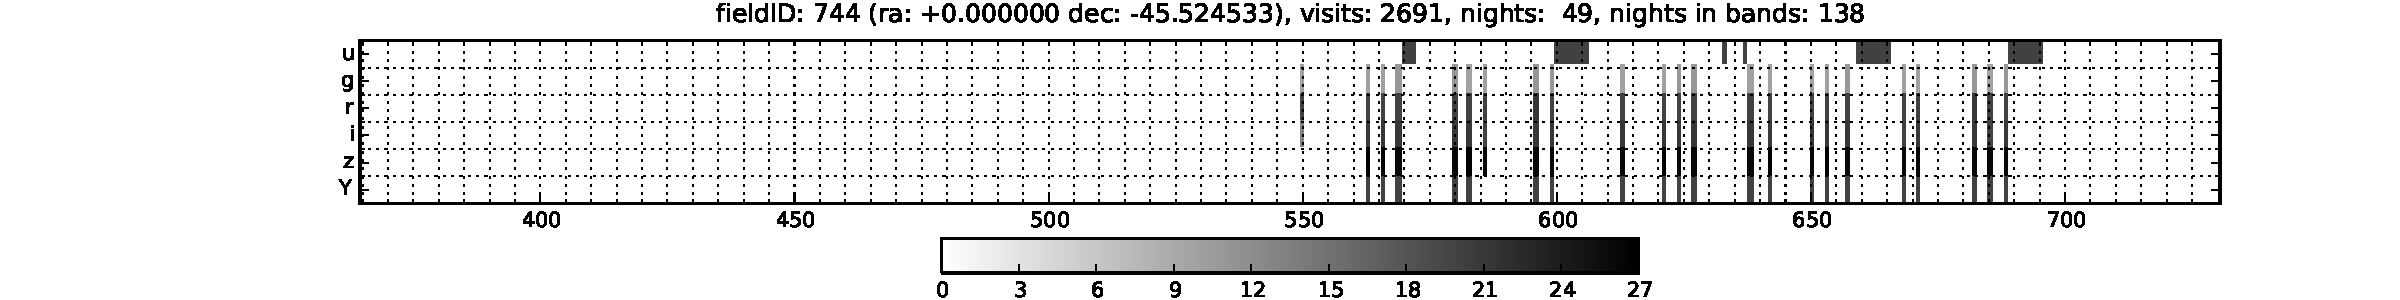
\includegraphics[width=\textwidth]{figs/supernova/fig_744_2ndYear}
 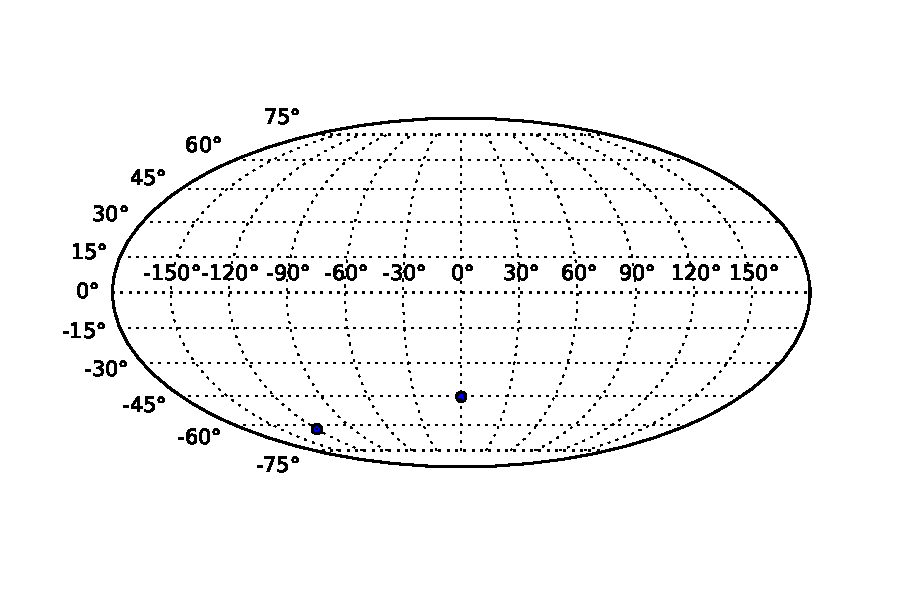
\includegraphics[height=0.2\textheight]{figs/supernova/loc_309_744.pdf}
 \label{fig:SN_sampling}
 \caption{Example of the cadence in the 2nd season in a WFD Field (fieldID 309) (top-panel) and a Deep Drilling Field (fieldID 744) (middle panel) and the
     spatial location of these two fields shown on a map. The cadence plots show a heatmap of the number of observations per night during the second season in each filter u, g, r, i, z, y. For viewing convenience a dotted grid is provided at an interval of 5 days. The header shows useful summary statistics:
 the fieldID and location of the field, the total number of visits during that period, the number of distinct nights on which observations are taken, and the number of distinct observations (where an observation are considered indistinct if they are on the same night and use the same band}
t
\end{figure}

 \begin{center}
\begin{figure}
 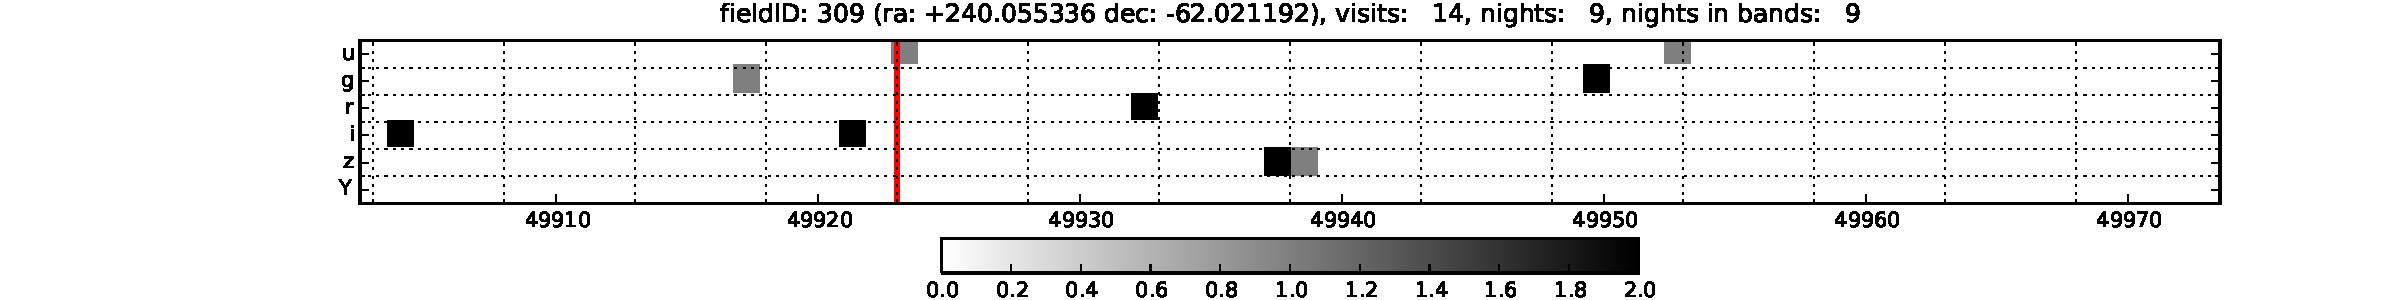
\includegraphics[width=\textwidth]{figs/supernova/TimeWindow_309_49923.pdf}
 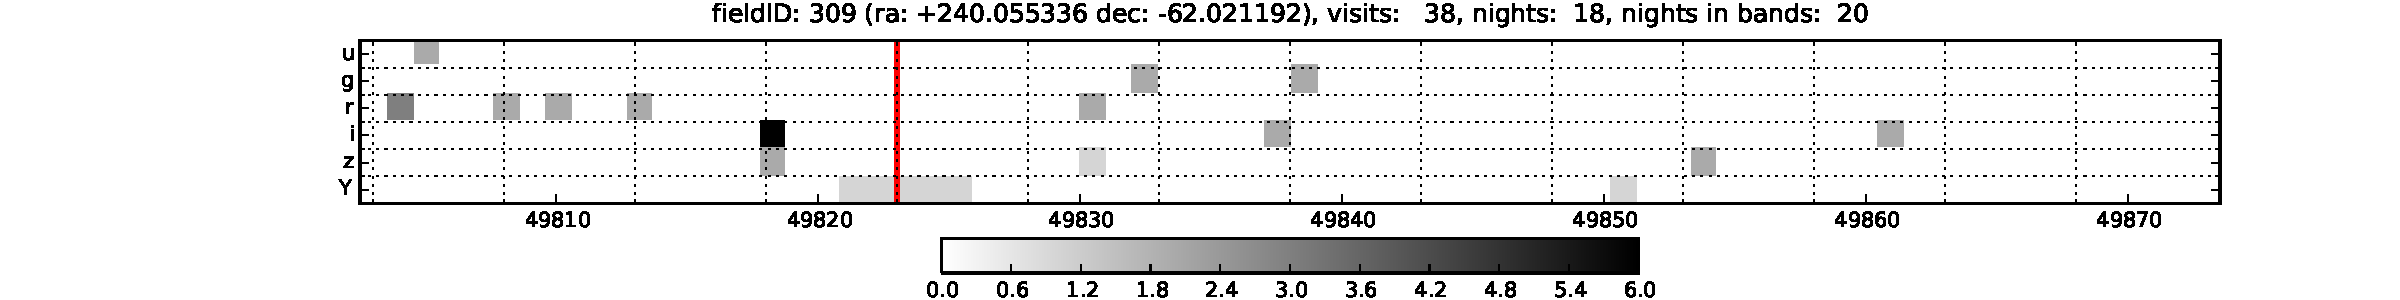
\includegraphics[width=\textwidth]{figs/supernova/TimeWindow_309_49823.pdf}
 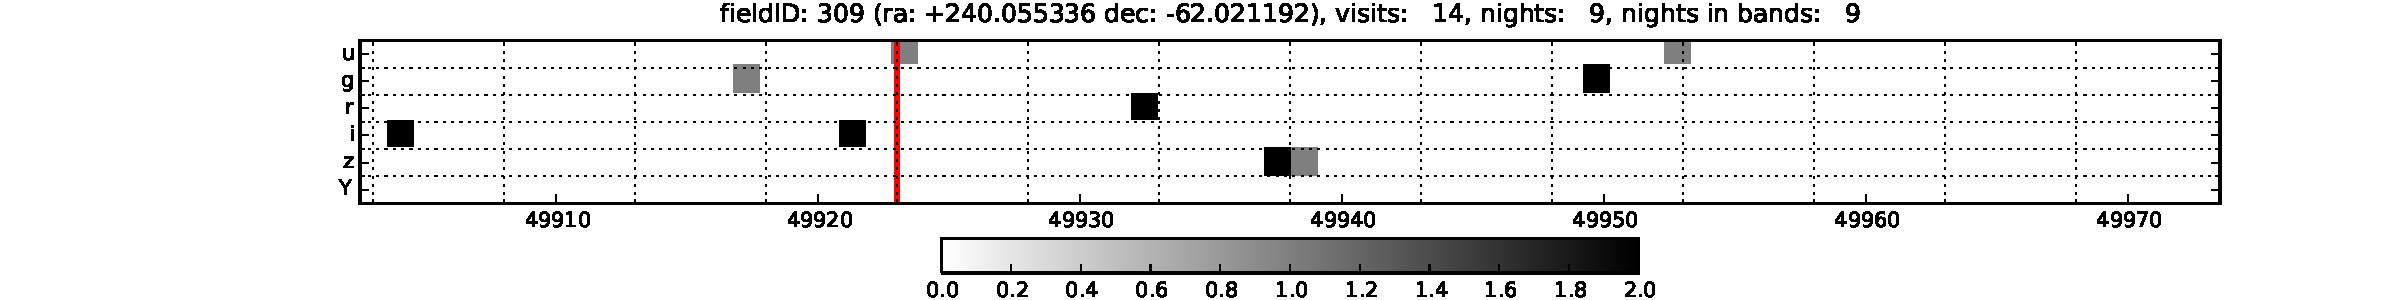
\includegraphics[width=\textwidth]{figs/supernova/TimeWindow_744_49923.pdf}
 %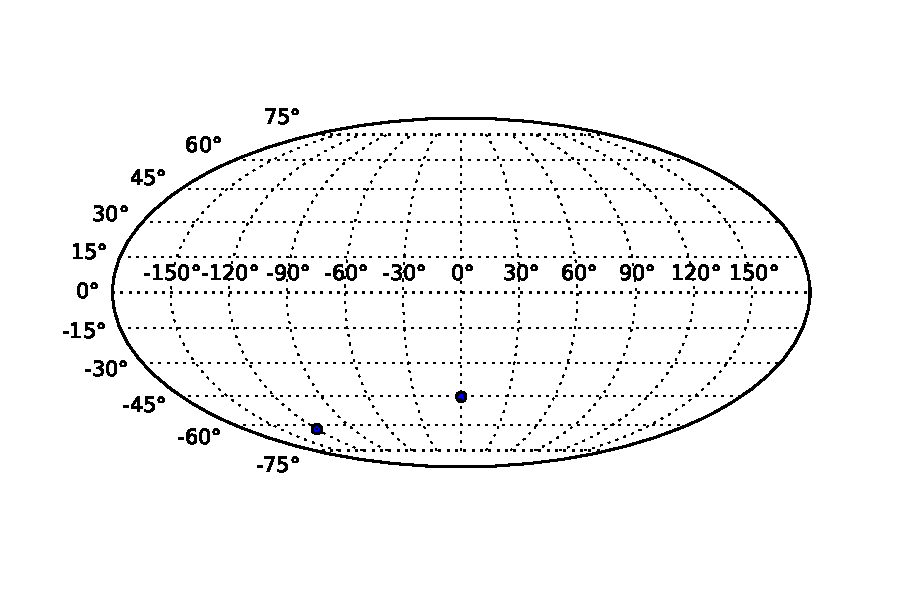
\includegraphics[height=0.2\textheight]{figs/supernova/loc_309_744.pdf}
 \label{fig:TimeWindow}
 \caption{Example of a TimeWindow in a WFD Field (fieldID 309) (top-panel) and a second TimeWindow (middle panel) on the same field, and a Deep Drilling Field (fieldID 744) (bottom panel) all extending -20 days before and 50 days after a chosen night or MJD. For the Deep Drilling Field in the bottom panel, and the WFD field in the top  panel, the chosen date around which the TimeWindow is constructed is the MJD of 49923, which is also 570 nights into the survey and marked by a red vertical line (which can be used to compare the location to Fig.~\ref{fig:SN_sampling}. The middle panel shows a window in Field 309 centered around an MJD of 49823 or a night of 470 which may also be compared to Fig.~\ref{fig:SN_sampling}. The plots again show the heatmap of observations in each filter in each night as in the cadence plots of Fig.~\ref{fig:SN_sampling}.}
\end{figure}
 \end{center}


Since the steps described above are all necessary for determination of SN intrinsic brightnesses, a metric for supernovae cosmology must quantify the ability to perform these steps on each supernova of the sample. To connect this to the output of OpSims, we could employ the following strategy:
\begin{itemize}
    \item study the sequences of observations in small spatial regions of the sky so that the sequences of observations relate to positions of astrophysical objects like supernovae. This capability is already built into \verb MAF ~ 
with multiple slicers like the \verb OpSimFieldSlicer ~ or the \verb Healpix ~ slicer. For example, in Fig.~\ref{fig:SN_sampling}, we show such a sequence for a WFD and DDF field for a single year (This is equivalent to using the
\verb OpSimFieldSlicer ~.)
    \item On each such spatial region, we look at sliding time windows, each time window of size about 70 days (corresponding roughly to a supernova Type Ia  lifetime starting 20 days before peak and extending to about 50 days after peak). As an example, we choose a time window around the night=570, which has
       an MJD value of 49923 for both the fields (fieldID: 744 and 309) 
       shown in Fig.~\ref{fig:SN_sampling} and show the timeWindow in Fig.~\ref{fig:TimeWindow}.
    \item  We assign a metric value that we call \textbf{perSNMetric} $PM$. 
        to each of these time-windows meant to estimate the quality of observations for a supernova whose rough lifetime matches that time window. The prescription for assigning these value to each time-window defines our metric and
 should quantify the success of the steps mentioned above.
 We would expect this value to be a function of the properties of the sequence of observations and the properties of the transients (SN) being studied.
 $$ PM = PM(\rm{observation Sequence, SN properties})$$
    \item We add up the \textbf{perSNMetric} for the time windows to estimate the metric values $M$ for the spatial region of the sky surveyed. 
        $$M = \sum_i PM_i $$
\end{itemize}



We will use two different approaches to defining the perSNMetric:
a. Use a simulated supernovae Type Ia with specific parameters, observed with the sequence of observations in the above time-window, and evaluate the success of each step.
b. Study heuristics of the observation sequences. We will provide some examples of this.

We will first discuss approach (a).
As the SN metric in a spatial region reflects the contribution of the sample
of SN observed in that spatial region towards inferring the cosmological
parameters. To warm up, consider a case where each SN observed with conditions better than a certain threshold contributes equally to the inference, the
relevant metric would be a function of the number of SN in the sample passing
such selection criteria. More generally, when the quality of all the supernovae are not similar enough, the metric should be thought of as the weighted sum of supernovae, with the weights being related to the inverse of the effective 
variance of the distance modulus.
\begin{equation}
M\sim \sum_i w_i , \qquad  w_i \sim 1.0 /\sigma^2_\mu
\end{equation}
By comparing with the form of the perSNMetric, we see that the perSNMetric
should be a proxy for $1.0/\sigma^2_\mu,$ where $\sigma^2_\mu$ is the effective variance on the measured distance modulus of the supernova.

%\subsubsection{ Steps in the PerSNMetric}
{\it  Steps in the PerSNMetric}

As described before, the measurement of the distance modulus is the result of several steps. Therefore, we expect the perSNMetric to be a product of metrics in each of the steps:

\begin{equation}
PM_i = \prod_{\rm{steps}} PM_i^{\rm{steps}}
\end{equation}

These components of perSNMetric constructed in different steps are described in Tab.~\ref{tab:stepsAndMetrics}
\begin{center}
 \begin{table}
\begin{tabular}{| p{5cm} |p{10cm}| }
\hline Metric & Description \\
\hline
I. SN discovery  &  Given the observations in a time window corresponding to the lifetime of a supernova, evaluate the  probability of detecting a
transient \\
II. SN classification & Given the observations in a time window corresponding to the lifetime of a supernova, evaluate the probability of classifying the transient\\
III. SN light curve characterization quality & Given the observations in a time window corresponding to the lifetime of a supernova, evaluate the quality of characterization\\
\hline \end{tabular}
\label{tab:stepsAndMetrics}
\end{table}
\end{center}



\subsubsection{I. Discovery Metric}
This metric is a proxy for the probability of detecting a SN as a transient
from the set of single epoch (visit) exposures during the lifetime of a supernova. Here we
assume that a single detection out of these visits is sufficient to identify the source as
a transient. This probability is constructed by comparing the probability of transient
detection for a point source of given SNR and filter band for a single visit and the set of SNR values of a supernova based on the observation sequences. 
This single
visit probability currently uses an approximation from previous surveys (in particular a SNR-efficiency curve constructed from the Dark Energy Survey, and
provided by R. Kessler, priv. communication).

\subsubsection{II. Classification Metric}
The classification metric is based on the output of the multifaceted machine learning 
classification system described in Section \ref{sec:\secname:targets}. For a given set of supernovae 
(simulated or real), we run the classification pipeline producing a probability of belonging to 
each class of supernova, for each object. The success of the classification can be evaluated in 
several ways. Here, to allow a general and robust metric, we use receiver 
operating characteristic (ROC) curves.\\
Most machine learning algorithms are capable of producing an estimate of the probability for each 
class, rather than just a single classification. Varying the threshold probability at which one 
considers an object belonging to a particular class can dramatically change the 
resulting classification. For example, requiring a threshold probability of 0.99 for an object to 
be considered a type Ia would result in an extremely pure Ia sample, albeit a rather small one as 
many objects would be missed. Thus classification problems always result in a trade-off between 
purity and completeness. This is illustrated by ROC curves (see Figure \ref{fig:roc}), where the 
false positive rate (contamination) is plotted against the true positive rate (completeness), as a 
function of probability threshold.\\
To understand true and false positive rate, consider the confusion matrix in Table 
\ref{table:confusion} for a binary classification problem. True positive rate (TPR) is then defined 
as
\begin{equation}
 \rm{TPR} = \frac{\rm{TP}}{\rm{TP}+\rm{FN}}
\end{equation}
and false positive rate (FPR) is defined as

\begin{equation}
 \rm{FPR} = \frac{\rm{FP}}{\rm{FP}+\rm{TN}}.
\end{equation}

Thus plotting the TPR against the FPR for varying probability threshold yields a ROC curve. 
Finally, the ROC curve can be summarised into a single number, although with some loss of 
information, by computing the area-under-curve (AUC), which is simply the integral under the ROC 
curve. The closer this number is to 1, the better the classifier in question is at returning a 
pure sample with high completeness. The AUC allows direct comparison between classifiers for a 
range of scenarios (i.e. not simply demanding a pure sample), making it a more general metric to 
use than accuracy, purity or efficiency and is the metric we use for the classification part of the 
supernova analysis.

\begin{table}
\centering
 \begin{tabular}{|c|c|c|}
 \hline
  & \multicolumn{2}{|c|}{True class}\\
  \hline
  Predicted class & Positive & Negative\\
  \hline
  Positive & True positive (TP) & False positive (FP)\\ 
  \hline
  Negative & False negative (FN) & True negative (TN)\\
  \hline
 \end{tabular}

 \label{table:confusion}
 \caption{Confusion matrix for a classification problem with two classes: positive (P) and negative 
(N).}
\end{table}


\begin{figure}
 \centering
 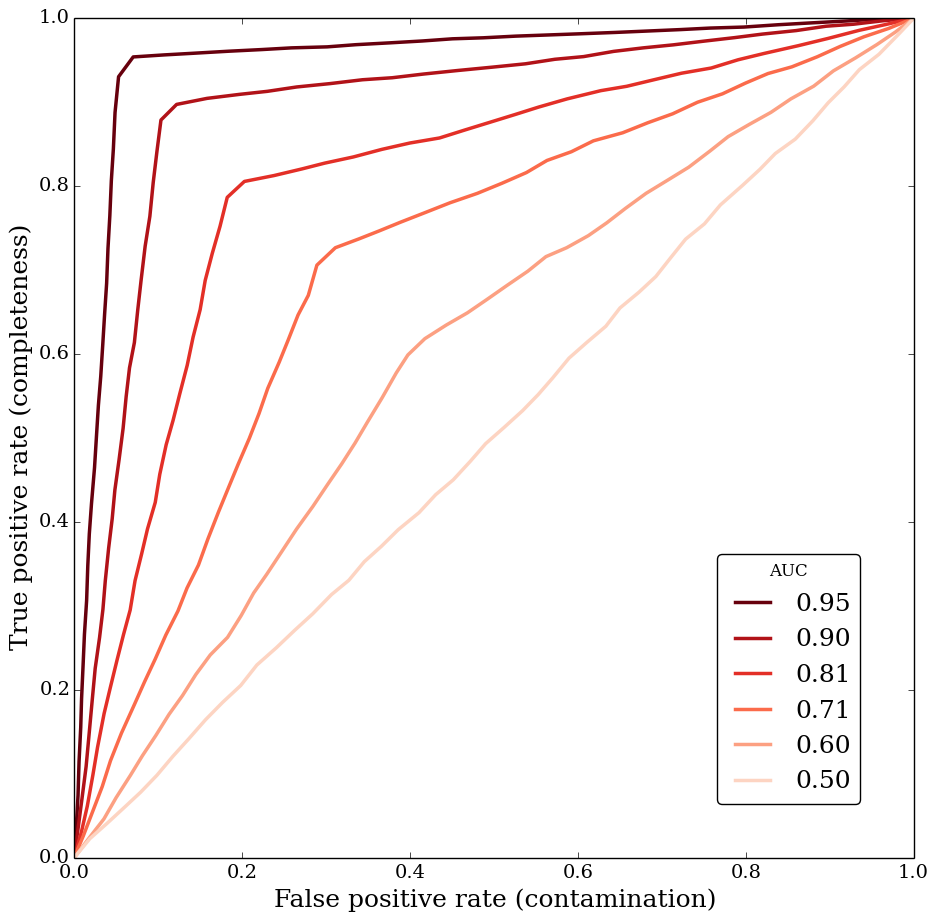
\includegraphics[width=0.7\hsize]{figs/supernova/roc_illustration}
 \label{fig:roc}
 \caption{An example receiver operative characteristic (ROC) curve. Each line plotted is an example 
classifier, ranging from bad (light-colored) to (dark-colored). The x-axis is false positive rate 
(contamination) and the y-axis is true positive rate (completeness) and the lines are plotted by 
varying threshold probability to produce different sets of classifications (see text for details).}
\end{figure}

\subsubsection{III. Quality Metric}
We construct the quality metric for the perSNmetric by obtaining the light curve of the SN
in the time window described above. We fit the light curve, and approximately estimate the
uncertainty in distance from the light curve fit alone. Of course, as is well known,
luminosity distance estimates of supernova Type Ia also show an intrinsic scatter of
around $0.1$ in previous surveys, which may be expected to decrease with better training
samples and understanding of underlying correlations of SNIa properties and their
environments. We compute a quality metric for each SNIa as the ratio of the square of the
uncertainty of the distance indicator from the supernova to the square of the intrinsic
dispersion. When added up over SN to obtain a value $QM$, the uncertainty on cosmological
parameters may be expected to scale as $\sim sqrt(1.0 + \sum QM)$ The quality metric evaluated on 
the example SN plotted is $1.$ if observed in the deep field, and $0.002$ in
the WFD field.




% --------------------------------------------------------------------

\subsection{OpsSim Analysis}
\label{sec:\secname:analysis}

{\bf Motivation and description:}

The scientific goal of characterizing SNe is to a large extent dependent on
how well the light curves of individual SNe are sampled in time and filters. To study
this, we re-index the OpSim output on spatial locations rather than use the temporal
index. Here we first
illustrate  in terms the cadence in an example LSST field. Our primary goal for optimal Observing
Strategy for SN observations is to obtain 7-10 epochs spread over 50 days or so for more than one filter {\it (we
will quantify the minimum filters later in the Section)}. This will increase the number of
well-measured SNe at low redshift (z$<$ 1) and improve distinguishing SN Ia from other
types of SNe.

{\bf Analysis, Results and Discussion}


\begin{figure}[tbh!]
%\vskip -1.3in
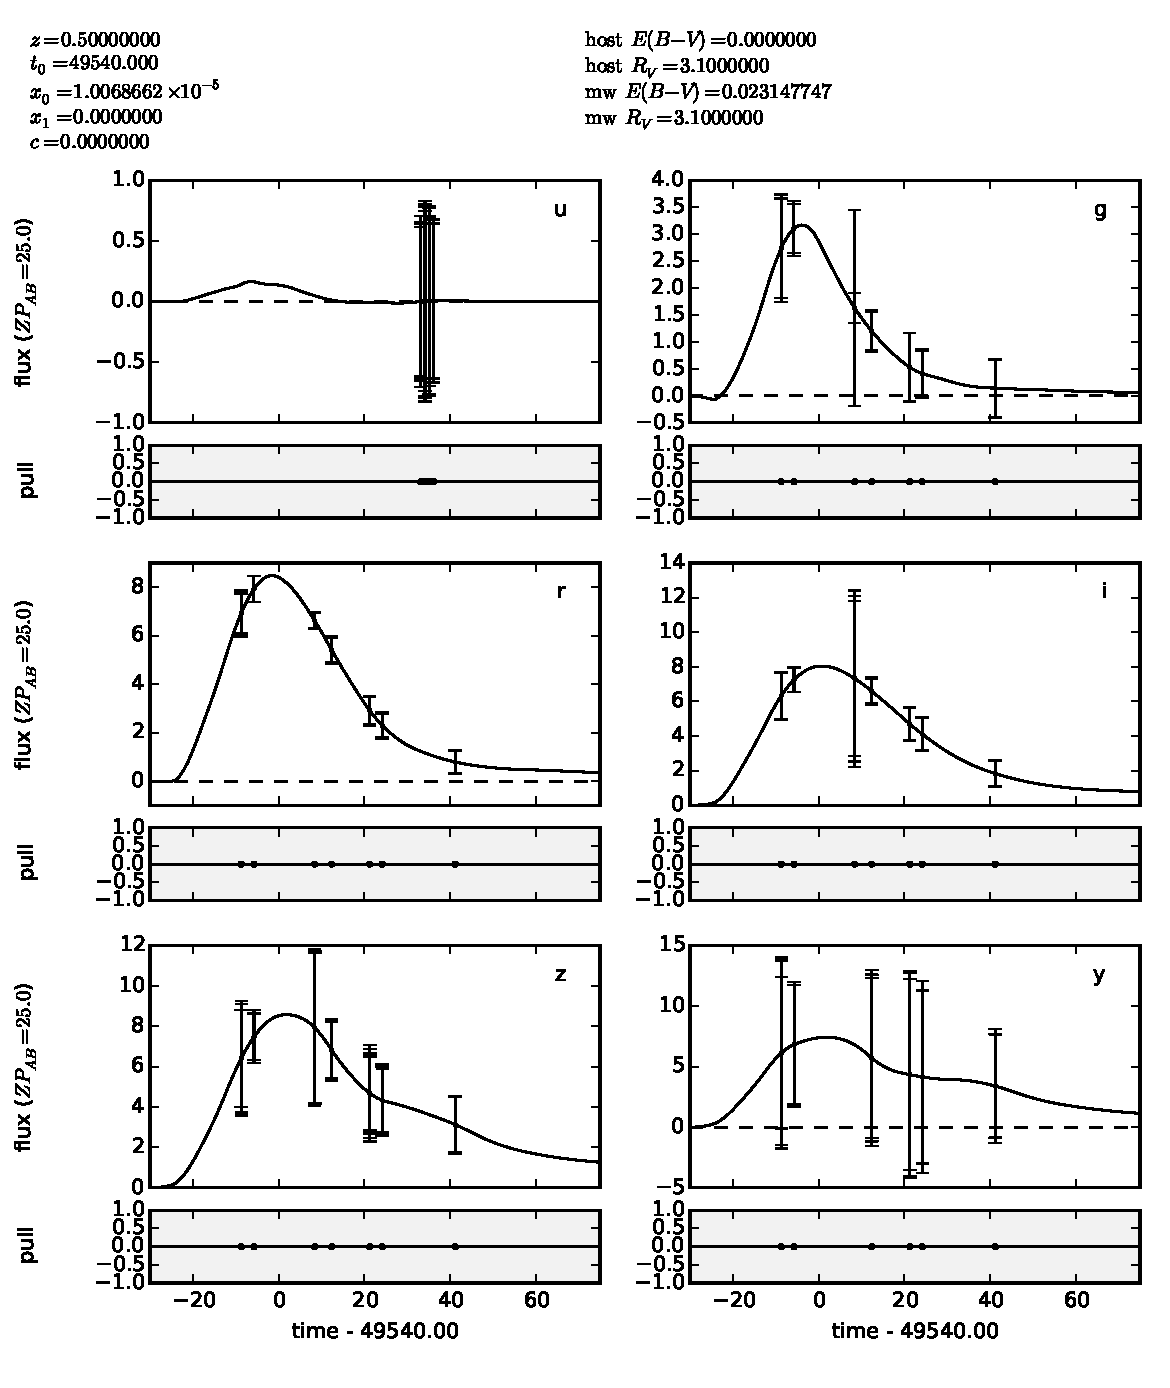
\includegraphics[angle=0,width=0.99\hsize:,clip]{figs/SN_290_lc.pdf}
%\vskip -1.3in
\caption{An example of light curve of SN Type Ia using Deep-Drilling Survey of the LSST Baseline OpSim run.
}
\label{fig:SNIaLCopsimdeep}
\end{figure}



\begin{figure}[tbh!]
%\vskip -1.3in
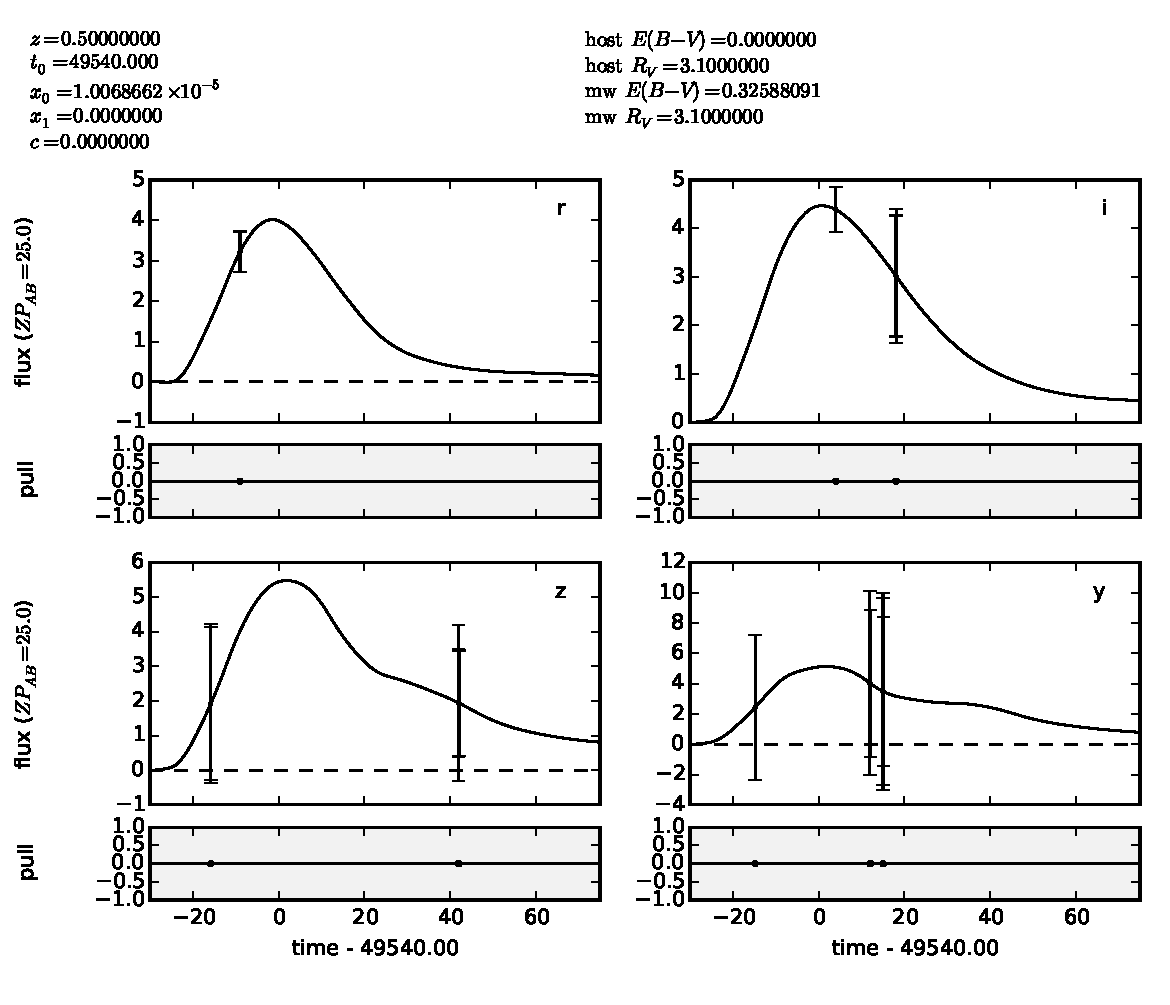
\includegraphics[angle=0,width=0.99\hsize:,clip]{figs/SN_309_lc.pdf}
%\vskip -1.3in
\caption{An example of light curve of SN Type Ia using the Main Survey of the LSST Baseline OpSim
run.
}
\label{fig:SNIaLCopsimmain}
\end{figure}

\begin{figure}[tbh!]
%\vskip -1.3in
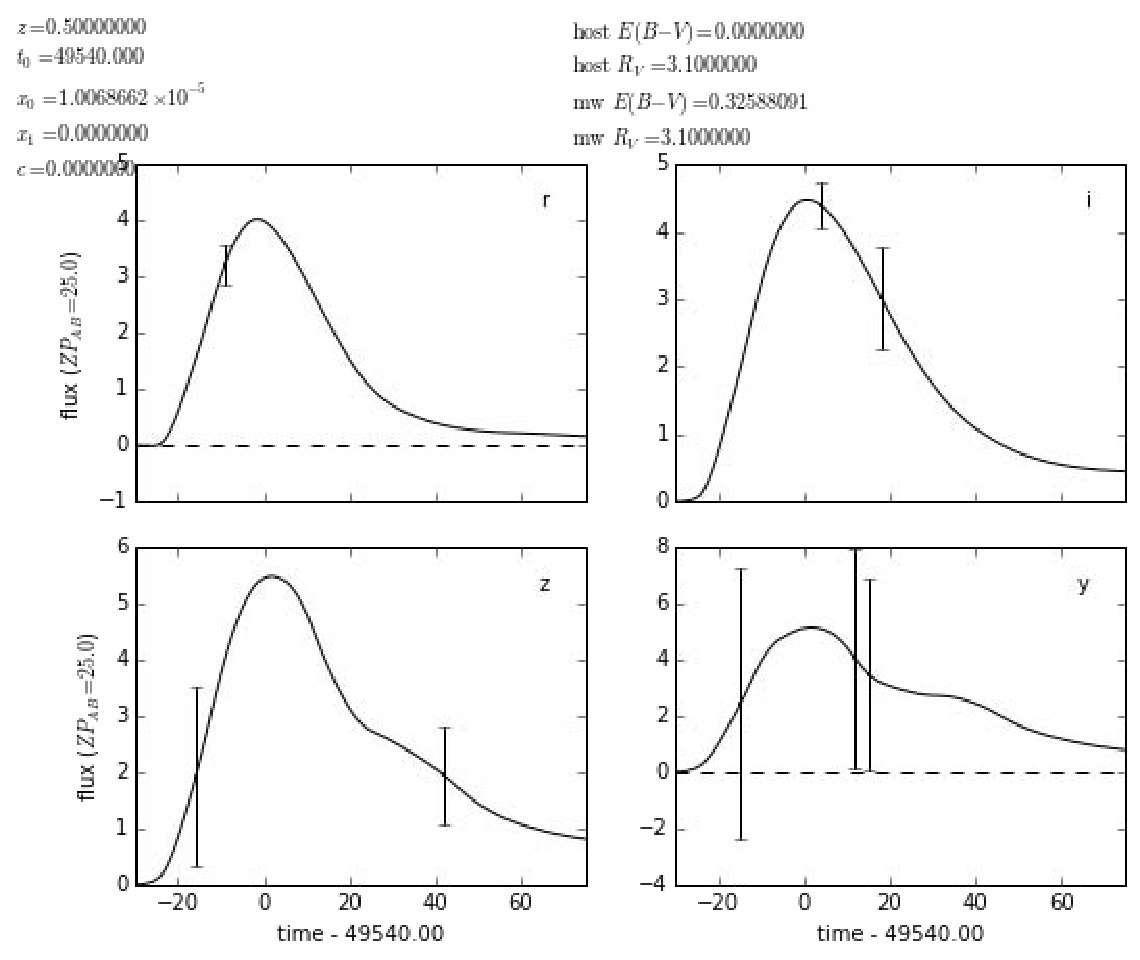
\includegraphics[angle=0,width=0.99\hsize:,clip]{figs/SN_309_lcavg.pdf}
%\vskip -1.3in
\caption{Time-interval averaged light curve of Figure \ref{fig:SNIaLCopsimmain}.
The light curve shows only a small number of the data points, which is insufficient
to classify this object as a Type Ia and may be also difficult to classify this object as
a SN. 
}
\label{fig:SNIaLCopsimmain2}
\end{figure}

We analyzed the OpSim output of the Baseline Observing Strategy,
enigma$\_$1189$\_$sqlite.db{\footnote {\url{http://ops2.tuc.noao.edu/runs/}}} using two sets of data: one using the Deep Drilling Fields and the other the main WFD survey. 
We generated light curves for a type Ia supernova with typical properties at a redshift of z=0.5 at few different locations using the observation sequences in the opsim output \verb enigma_1189 ~at those locations around a chosen date for peak. This date was chosen so that the 
sequence of observations is representative of good cadence in \verb enigma_1189 ~at that location. To do this, we used the SALT2-extended model with $x1, c=0$ and $x_0 $ set so that the SNIa would have a specific magnitude of $-19.3$ 
 in the rest frame BessellB band. This was performed using a version of SNCosmo to interpolate the SALT2 surfaces, and the LSST catalog simulation package
 to calculate the flux for LSST bandpasses.
Figure \ref{fig:SNIaLCopsimdeep} shows light curves in different
filters towards a deep drilling field (RA., Decl.). The number of visits for 50 days is 53
per filter. Using this light curve, we estimated both the quality metric and the discovery metric, and find that the both of the metrics are individually 1.
indicating that this is a transient that will be almost definitely 
discovered, the light curves will be of high enough quality to contribute extremely well to the inference of cosmological parameters. The light curves and quantified Metric demonstrate that data from Deep Drilling Fields
would generate high quality light curves, allowing a high rate of supernova discovery.

In contrast, a light curve from the Main Survey in Figure \ref{fig:SNIaLCopsimmain} is
somewhat limited. 
This light curve is generated towards Field 290 (R.A. of 6.097$^{\circ}$
and Decl. of -1.105$^{\circ}$; see Figure \ref{fig:perSNCadence}). An average number of
data points in the light curve is 2 per filter. Using this light curve, the probability we
 estimated this object to be a SN is less than 0.1. 

\emph{To be added: 2 more examples of light curves at different positions of sky.}




%OpSim analysis: how good would the default observing strategy be, at
%the time of writing for this science project?



\begin{figure}[tbh!]
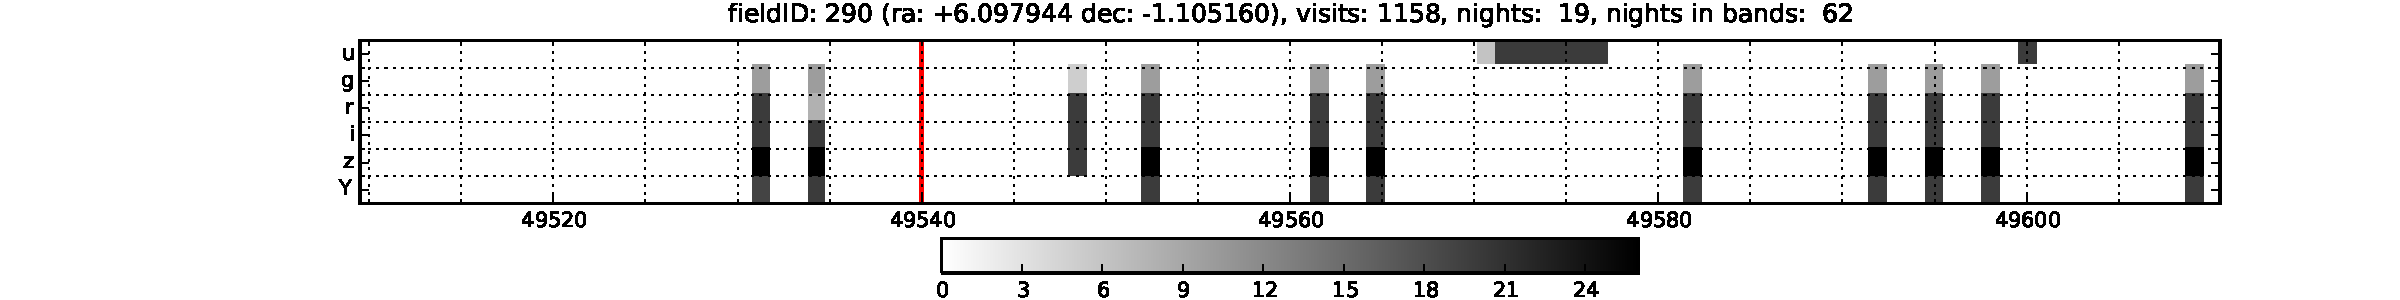
\includegraphics[angle=0,width=\textwidth,clip]{figs/SN_Cadence_290.pdf}
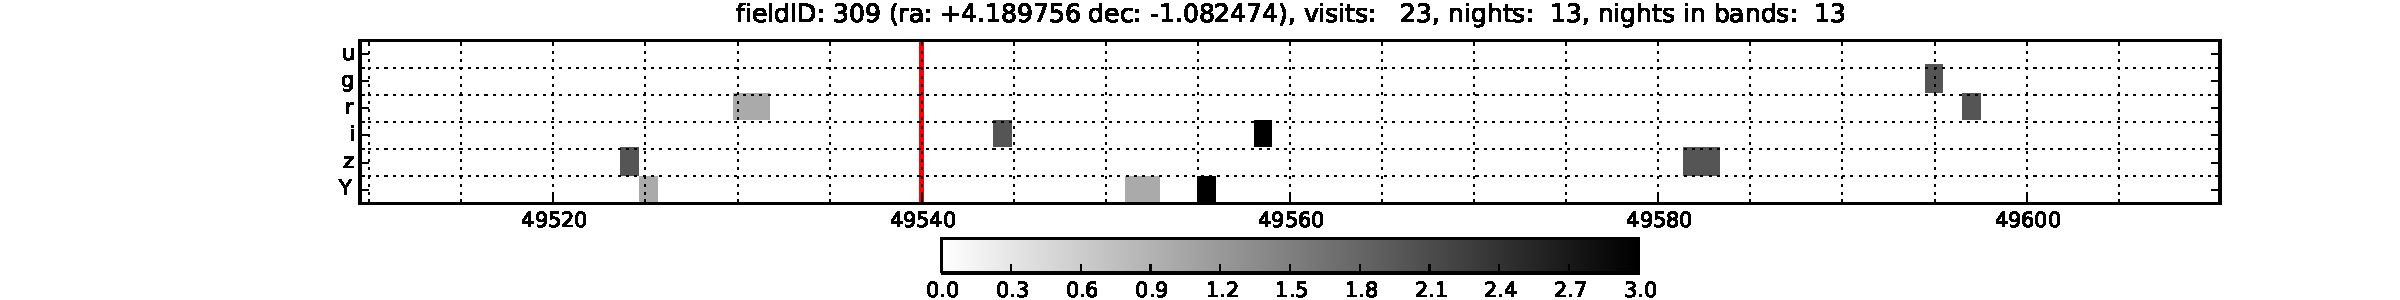
\includegraphics[angle=0,width=\textwidth,clip]{figs/SN_Cadence_309.pdf}
\caption{Cadence of Observations in the timewindow of a representative supernova at redshift of $z=0.5$ in a DDF (top) field (fieldID: 290) and a WFD (bottom) field (fieldID: 309). The red lines show the date of explosion, and the shades show the number of observations in a night in a distinct filter.}
\label{fig:perSNCadence}
\end{figure}



\begin{figure*}[!hb]
    \begin{minipage}[b]{\linewidth}
        \includegraphics[width=\textwidth]{figs/supernova/fig_firstSeason_0}
        \includegraphics[width=\textwidth]{figs/supernova/fig_firstSeason_1}
        \includegraphics[width=\textwidth]{figs/supernova/fig_firstSeason_2}
        \includegraphics[width=\textwidth]{figs/supernova/fig_firstSeason_3}
        \includegraphics[width=\textwidth]{figs/supernova/fig_firstSeason_4}
    \end{minipage}
\label{fig:opsimSummary}
\caption{Cadence of Observations in the timewindow of a year towards a few sample of 
positions. Grey-scale indicates the number of visits. {\it add details} 
}
\end{figure*}


% --------------------------------------------------------------------
\subsection{Rolling Cadence of the Main Survey Optimized for Supernova Science}
\subsubsection{ Scientific Motivation for Rolling-Cadence}

The main survey is important for the discovery of supernovae (SNe) in the redshift range of
0.1- 1, which is critical to constraint SN cosmological parameters. In order to identify a
variable source as a SN and to distinguish the source as a Type Ia SN, we need 7-10 epochs
spread over 45 days or so for each filter based on past experience. Universal survey of
the Baseline Cadence provides 6 filter data for approximately 18 days (assuming a survey with
a filter can be done for 3 days). This provides 15 data points over 45 days and 2.5 data
points in average for each filter. Our analysis of OpSim run (Baseline Observing Strategy)
output shows the light curves of SNe from the OpSim data are insufficient not only to
identify the source as a SN and but also to classify the SN if the SN is type Ia or II (or
Ib, Ic). Our proposed observing strategy is critical to improve the quality of SN light
curves. The light curves will have at least 3 times densely populated data points in time. 

\subsubsection{Proposed Rolling-Cadence of the Main Survey Optimized for SN Science }
%\label{sec:\secname:discussion}


{\it Discussion: what risks have been identified? What suggestions could be
made to improve this science project's figure of merit, and mitigate
the identified risks?}

Our goal for observing strategy optimized for SN cosmology is to
obtain 7-10 epochs spread over 50 days or so for more than one filter. We suggest to
change the filter every day and LSST can choose a part of sky which has the best airmass,
centered on Zenith. LSST will observe about 1/3 of visible sky per day (to be confirmed).
LSST can observe the same part of sky for 6 days with 6 filters, and repeat 9 times for
the same field. This observing strategy will result in 54 visits (with 6 different
filters) for the same field. We repeat the same for Field 2 which takes another 54 days.
Then observe Field 3 for another 54 days.

We propose a new Observing Strategy of the main survey in order to generate densely
populated SN light curves (3 times more densely populated data acquisition in time). For
simplicity, we assume the LSST main survey will cover the entire LSST fields for 3 days
(we divide the entire LSST fields into 3 separate fields, which would be called Field 1
and 2 and 3. The sum of Field 1 and 2 and 3 is the LSST entire fields) . For a day, 1/3 of
the LSST entire field would be observed. By changing the filter, every day, LSST can
observe 6 filters for 1/3 of the LSST entire fields. We repeat 9 times for the same field,
which will result in 54 visits (with 6 different filters) for the same field (1/3 of the
LSST entire fields). We repeat the same for Field 2 which takes another 54 days. Then
observe Field 3 for another 54 days. To visualize this idea, I list proposed observing
strategy day by day; Day 1 : Filter 1 (for Field 1), Day 2: Filter 2 (for Field 1), Day 3:
Filter 3 (for Field 1), Day 4: Filter 4 (for Field 1), Day 5: Filter 5 (for Field 1), and
Day 6: Filter 6 (for Field 1). Repeat this sequence 9 times for the Field 1. This will
generate 54 data points for 54 days for a supernova and average 9 data points for each
filter. Observe the same sequences for Field 2 (it takes 54 days) and then do the same for
Field 3 (it takes another 54 days). This summarizes overall idea, but since the visible
sky is different every day and the observation depends on the weather, an OpSim run is
needed accounting for all of these factors (and maybe others that we haven't mentioned
here). We have requested OpSim run based on the strategy described here.

\subsubsection{Expectations} 

\begin{enumerate}
\item SN light curves would have 3 times more densely populated in time as we have designed.
\item An average airmass of the Main Survey would be significantly lower.
\item Significantly higher number of SN discovery can be expected because its impact area is
large. The average number of visits per filter for 50 days is only $\sim$2 for the regions
located from Dec. -65 to Dec. 0 based on Baseline Observing Strategy, but the number would
be $\sim$6 with our proposed rolling cadence.
\end{enumerate}



%\begin{figure}[tbh!]
\begin{figure}
\vskip 3truecm
%\vskip -1.3in
%\includegraphics[angle=0,width=0.99\hsize:,clip]{figs/SNIaLCopsim.pdf}
%\vskip -1.3in
\caption{Predicted light curves of Supernova Type Ia using Rolling-Cadence. We used ramdom generation of time sequence.
}
\label{fig:SNIaLCopsimmainnew}
\end{figure}



\begin{itemize}
\item Intrinsic Dispersion, environmental effects, newer analysis methods 
\item Follow-up
procedures: What is feasible? Where will our training samples for classification and light
curve models come from (other experiments, our own sub-samples with spectroscopic
follow-up?), spectroscopic follow-up of host galaxies. Can hosts be identified? 
\item `Systematics': In what ways will the real data not match the assumptions made in analysis.
Having a large sample of SN, to understand the astrophysics would be useful for this. 
\end{itemize}


% ====================================================================

\navigationbar
